\documentclass[11pt,a4paper]{article}
\usepackage[T1]{fontenc}
\usepackage[utf8]{inputenc}
\usepackage[margin=1.9cm]{geometry}
\usepackage{amsmath,amssymb}
\usepackage{enumitem}
\usepackage{graphicx}
\usepackage{booktabs}
\usepackage{xcolor}
\usepackage{hyperref}
\usepackage{caption}
\usepackage{titlesec}

\hypersetup{colorlinks=true,linkcolor=blue,urlcolor=blue}
\graphicspath{{results/report_figs/}}

\titlespacing*{\section}{0pt}{0.9em}{0.35em}
\titlespacing*{\subsection}{0pt}{0.6em}{0.2em}
\titleformat{\section}{\normalfont\large\bfseries}{\thesection}{0.6em}{}
\titleformat{\subsection}{\normalfont\bfseries}{\thesubsection}{0.5em}{}
\captionsetup{font=small,skip=3pt}

\setlength{\parskip}{0.35em}
\setlength{\parindent}{0pt}
\setlength{\textfloatsep}{8pt}
\setlength{\intextsep}{8pt}
\setlength{\abovecaptionskip}{3pt}

\title{\vspace{-2.3em}\textbf{0--k BFS: Bounded Integer Weights Shortest Path Problem}\\
\normalsize Stage~1 Report -- Algorithms Course, C++ Implementation}
\author{Artemov Makar, Mark Shkut \quad\textit{Skoltech, Algorithms 2026}}
\date{\vspace{-0.6em}May 21, 2026}

\begin{document}
\maketitle
\vspace{-2em}

\section{Scope and deliverables}

We build and benchmark a C++ implementation of the 0--k BFS family of
shortest-path algorithms and compare it against a Dijkstra baseline, scaling
to the largest vertex count a commodity workstation can handle -- our target
was $V$ approaching $10^9$. At that scale explicit edge storage is infeasible
(a CSR with $E=4V$ and 32-bit ids/weights costs $\approx 20$\,GB at $V=10^9$),
so the project distinguishes two graph backends: \texttt{GridGraph} (implicit
4-neighbour grid + per-vertex byte, up to $V \approx 10^9$) and
\texttt{GraphCSR} (classical CSR, up to $V \approx 10^8$). The grid backend
never materializes edges; \texttt{for\_each\_neighbour(u)} runs in $O(1)$.
The dominant memory cost is the distance array, halved from 8\,GB
(\texttt{uint64\_t}) to 4\,GB (\texttt{uint32\_t}) because $k\cdot V < 2^{32}$
holds for every parameter we use.

\textbf{Deliverables:} (i)~four dataset generators (grid, ER, layered DAG,
chain with chords); (ii)~visualization (per-graph distance field + benchmark
plots); (iii)~pipeline runner with JSONL output; (iv)~Dijkstra baseline;
(v)~0--1 BFS and 0--k BFS (with $k{+}1$ circular FIFO queues).
Every algorithm's distance checksum was verified against Dijkstra on
identical inputs; all 19 distinct graph instances from the 45-run parameter
sweep cross-validate (zero mismatches).

\section{Algorithms}

\textbf{(a) \texttt{dijkstra\_pq} (baseline).} Standard Dijkstra with
\texttt{std::priority\_queue} and lazy decrease-key (push duplicates, skip
stale pops). $O((V+E)\log V)$.\\
\textbf{(b) \texttt{bfs\_01}.} \texttt{std::deque<Vertex>}: weight 0
$\to$ \texttt{push\_front}, weight 1 $\to$ \texttt{push\_back}. $O(V+E)$.\\
\textbf{(c) \texttt{bfs\_0k}.} $k{+}1$ circular FIFO queues indexed by
$dist[v] \bmod (k{+}1)$; the current processing distance \texttt{cur} walks
forward, vertices re-relaxed land in another bucket, stale slots are skipped
on pop. $O(kV+E)$, memory $O(k+E)$ for the queues plus $O(V)$ for
distances. All three are templated over a graph adapter, so the same code
runs on both backends.

\section{Datasets and visualization}

Four generators with seeded \texttt{std::mt19937\_64} RNG:
\texttt{grid} (rows, cols, $k$ -- the headline case for $V \to 10^9$),
\texttt{er} ($G(n,p)$, weights $\in \{0..k\}$),
\texttt{layered} ($L$ layers of width $W$, fanout $F$),
\texttt{chain} (path of $n$ vertices $+ c$ random chords -- adversarial).
For the grid, $w(u,v) = (\mathrm{terrain}[u] + \mathrm{terrain}[v]) \bmod (k{+}1)$
produces structured weight landscapes that show up clearly in the heatmap
(Fig.~\ref{fig:viz}, left). Two visual layers come from JSON emitted by
\texttt{zkbfs\_dump}: per-graph distance fields (grid heatmap or node-link
with colour~$=$~distance) and benchmark plots aggregated from the JSONL
sweep.

\begin{figure}[h]
\centering
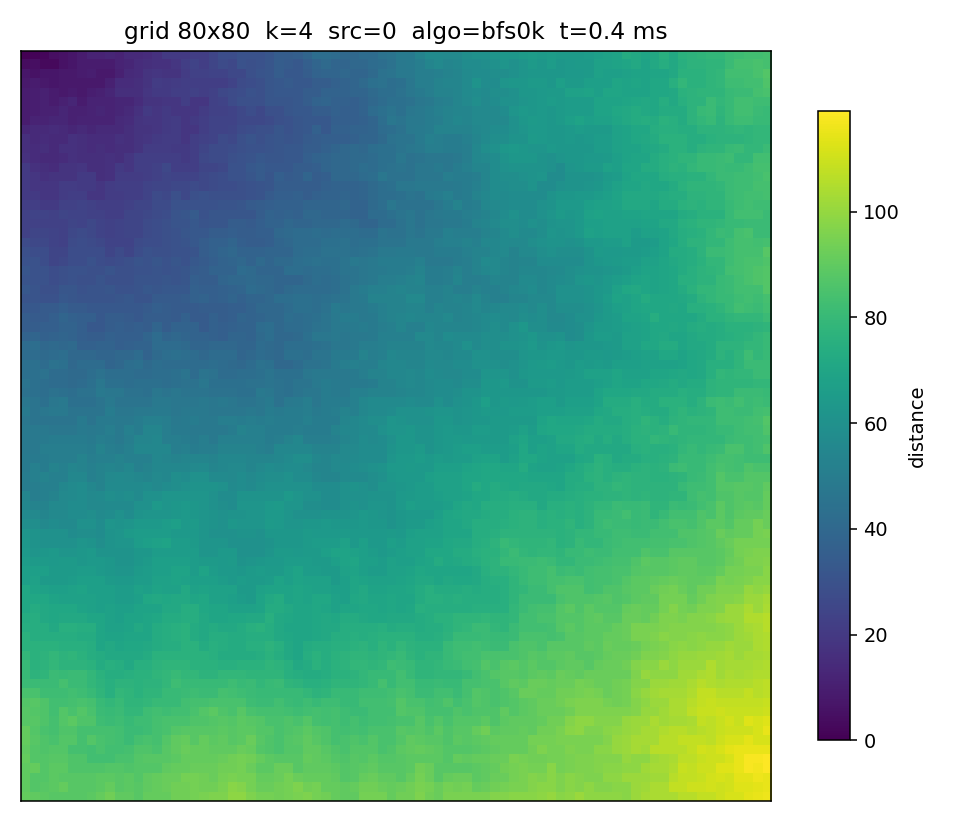
\includegraphics[width=0.42\linewidth]{viz_grid_heatmap.png}\hspace{0.7em}
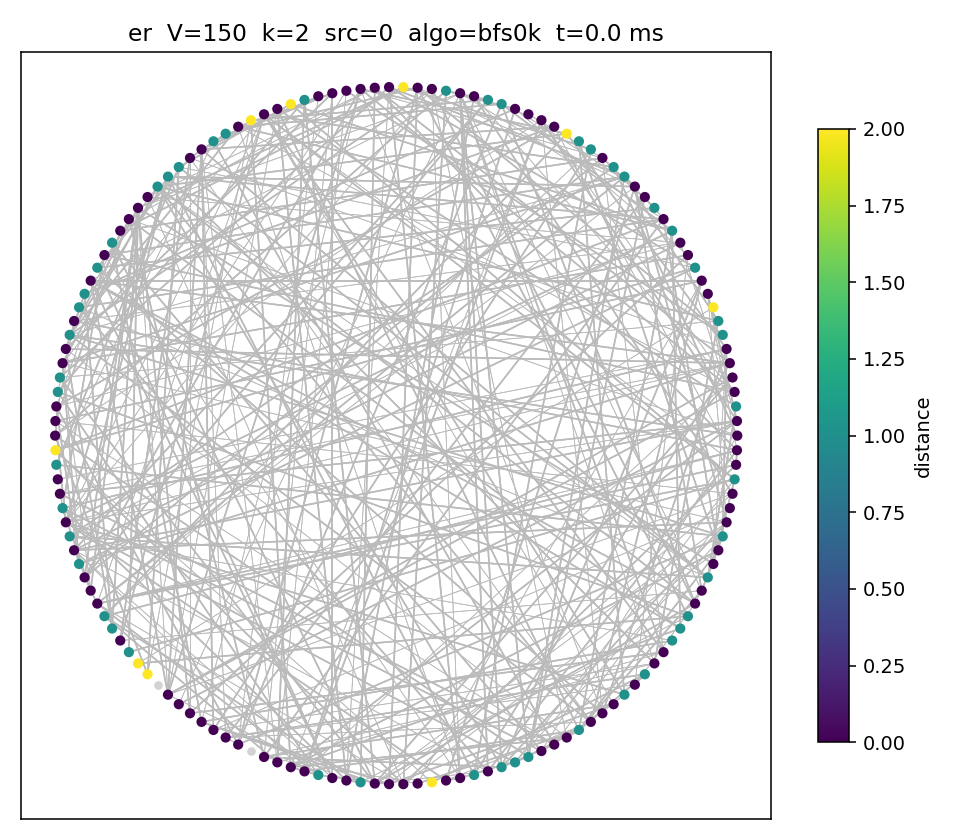
\includegraphics[width=0.40\linewidth]{viz_er_nodes.png}
\caption{\textbf{Left:} $80{\times}80$ grid, $k=4$, source at the top-left;
the heatmap shows the distance field shaped by random terrain.
\textbf{Right:} Erdős--Rényi graph, $V=150$, $p=0.03$, $k=2$; edges in grey,
vertex colour encodes distance from the source.}
\label{fig:viz}
\end{figure}

\section{Results}

\begin{figure}[h]
\centering
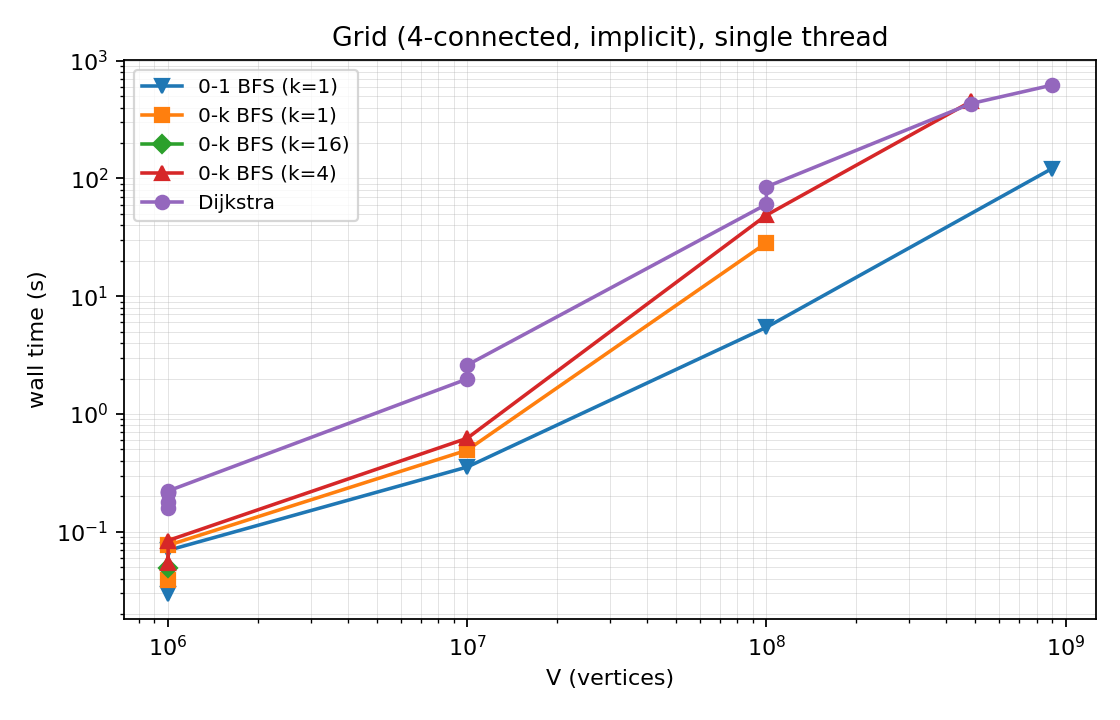
\includegraphics[width=0.49\linewidth]{grid_scaling.png}\hfill
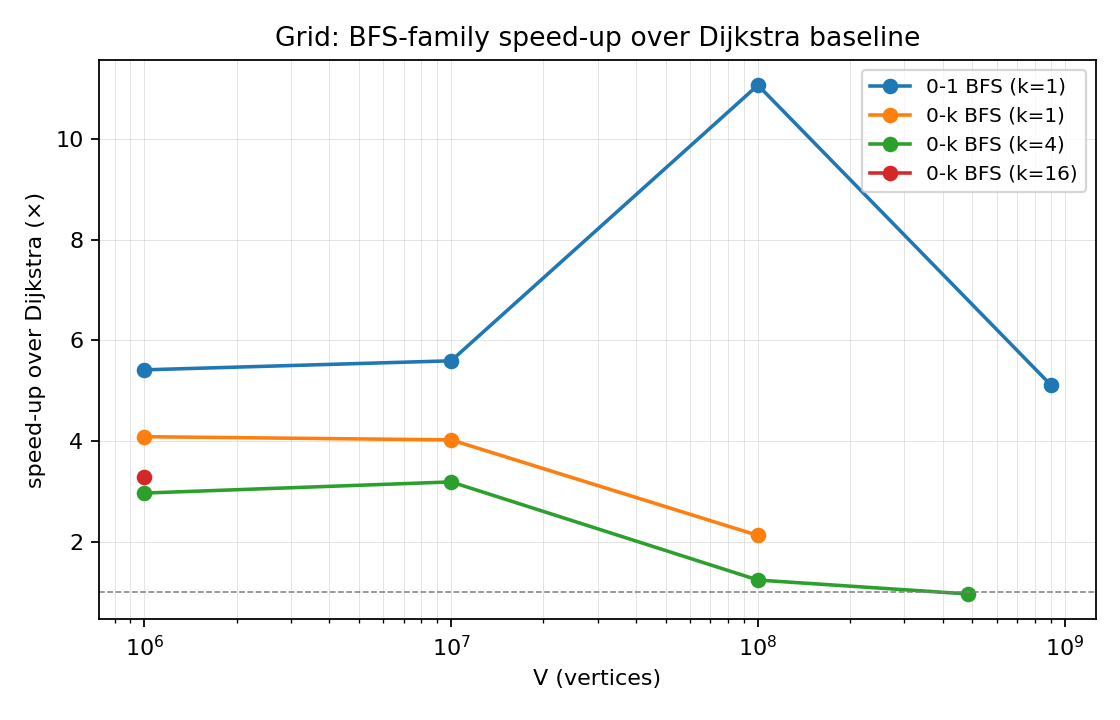
\includegraphics[width=0.49\linewidth]{speedup_vs_V.png}
\caption{Implicit 4-connected grid, single thread.
\textbf{Left:} wall time vs $V$ (log--log).
\textbf{Right:} BFS-family speed-up over the Dijkstra baseline; the dashed
line marks parity. The 0--1 BFS via \texttt{std::deque} peaks at
$\sim 11\times$ at $V=10^8$ before memory pressure pulls it back.}
\label{fig:results}
\end{figure}

\textbf{Headline numbers (grid, single thread).}
\begin{center}
\small
\begin{tabular}{rrrrrl}
\toprule
$V$            & $k$ & Dijkstra & 0--k BFS & 0--1 BFS & best speed-up \\ \midrule
$10^6$         & 1   & 0.180\,s & 0.039\,s & 0.070\,s & $4.6\times$ \\
$10^6$         & 4   & 0.222\,s & 0.054\,s & ---      & $4.1\times$ \\
$10^7$         & 1   & 1.98\,s  & 0.493\,s & 0.355\,s & $5.6\times$ \\
$10^7$         & 4   & 2.61\,s  & 0.623\,s & ---      & $4.2\times$ \\
$10^8$         & 1   & 60.3\,s  & 28.4\,s  & 5.44\,s  & $\mathbf{11.1\times}$ \\
$10^8$         & 4   & 84.9\,s  & 48.8\,s  & ---      & $1.7\times$ \\
$4.84\cdot 10^8$ & 4 & 432.9\,s & 451.4\,s & ---      & $0.96\times$ (mem-bound) \\
$9\cdot 10^8$  & 1   & 619.9\,s & ---      & 121.2\,s & $\mathbf{5.12\times}$ \\
\bottomrule
\end{tabular}
\end{center}

\textbf{V$\approx 10^9$.} The largest run used a $30\,000{\times}30\,000$
implicit grid ($V=9\cdot 10^8$, $E=3.6\cdot 10^9$). Single thread, commodity
RAM: Dijkstra $619.9$\,s, 0--1 BFS $\mathbf{121.2}$\,s -- speed-up
$\mathbf{5.12\times}$. Both produce the same distance-sum checksum
$1\,703\,472\,107\,894$, so correctness holds at the billion-vertex scale.
Working set during the 0--1 BFS run was $\approx 8.5$\,GB: $3.6$\,GB for
the \texttt{uint32\_t} distance array, $0.9$\,GB for the terrain,
$\approx 4$\,GB peak for the \texttt{std::deque} of pending vertices.

\section{Limitations and observations}

\textbf{Crossover with $k$.} As $k$ grows the 0--k BFS speed-up shrinks:
the $V=10^6$ grid shows $4.6\times$ at $k=1$, $4.1\times$ at $k=4$,
$3.3\times$ at $k=16$. Asymptotically the advantage disappears at
$k = \omega(\log V)$.\\
\textbf{Memory-bandwidth ceiling.} At $V \gtrsim 5\cdot 10^8$ both
algorithms become memory-bound: the queues alone are multi-gigabyte
structures (peak push count $\approx 6\cdot 10^8$), so the algorithmic
advantage of 0--k BFS over a cache-friendly Dijkstra essentially vanishes
(the $V=4.84\cdot 10^8$ row is $0.96\times$). The 0--1 BFS via a single
\texttt{std::deque} stays competitive at $V=9\cdot 10^8$ because a deque
is chunked and noticeably more cache-friendly than $k{+}1$ separate queues.\\
\textbf{Implementation cost of \texttt{std::queue}.} At $V=10^8, k=1$ the
single-deque 0--1 BFS runs in $5.4$\,s vs. the two-queue 0--k BFS at
$28.4$\,s. Same algorithmic complexity -- the gap is pure allocator/cache
overhead of maintaining $k{+}1$ FIFOs. A chunked ring-buffer FIFO is the
planned Week~2 fix.\\
\textbf{Lazy decrease-key.} Our Dijkstra reinserts entries instead of
supporting \texttt{decrease\_key}; an indexed $d$-ary heap is queued for
Week~2.

\section{Next steps (Week 2)}

(1)~Indexed 4-ary heap Dijkstra; rerun the headline grid sweep.
(2)~Chunked ring-buffer FIFO in \texttt{bfs\_0k} to close the gap against
the deque-based 0--1 BFS.
(3)~Real road-network loader (DIMACS USA, weights quantised to $k=8$).
(4)~Stretch goal: a $\Delta$-stepping variant for context (parallel friendly).

\end{document}
